\documentclass{genai}

\title{Homework 2 Writeup}
\author{Due: Friday I think}
\date{}



\begin{document}

\head{CSCI-297}{Generative AI}

\renewcommand{\labelenumii}{\arabic{enumi}.\arabic{enumii}}
\renewcommand{\labelenumiii}
{\arabic{enumi}.\arabic{enumii}.\arabic{enumiii}}
\pagestyle{fancy}
\newpage

\maketitle

\subtitle

\newpage

\section{Model Architecture}

There are two classes, Generator and Discriminator, which are key components of a Generative Adversarial Network (GAN).
GANs are a type of neural network architecture used for generating new data that resembles the input data.

\textbf{Generator}: This class is responsible for generating new data. It takes a latent vector (a random noise) as input and outputs an image.\
The architecture of the generator model is a series of linear layers (nn.Linear), each followed by a LeakyReLU activation function (nn.LeakyReLU) and batch normalization (nn.BatchNorm1d).
The final layer is a Tanh activation function (nn.Tanh), which scales the output to be between -1 and 1.

\textbf{Discriminator}: This class is responsible for classifying whether a given image is real (from the dataset) or fake (generated by the generator).
It takes an image as input and outputs a single value representing the probability that the image is real.
The architecture of the discriminator model is a series of linear layers (nn.Linear), each followed by a LeakyReLU activation function (nn.LeakyReLU).
The final layer is a Sigmoid activation function (nn.Sigmoid), which scales the output to be between 0 and 1, representing the probability.

Both classes inherit from nn.Module, which is a base class for all neural network modules in PyTorch.
This means they both must implement a forward method that defines how to compute the output using the layers defined in the \_\_init\_\_ method.

\section{Training Process}

Training a GAN involves training the generator and discriminator models simultaneously.
To train the GAN, I used the following processes:

\begin{algorithm}[h]
    \caption{GAN Training}
    \begin{algorithmic}[1]
        \Procedure{Train Discriminator}{$D$, $G$ loss\_fn, $D_\text{optimizer}$}
            \State {fake\_images $\gets$ $G(\text{random\_noise})$}
            \State {real\_images $\gets$ images from dataloader}
            \State {predicted $\gets$ mapping of real\_images to $D(\text{real\_images})$, fake\_images to $D(\text{fake\_images})$}
			\State {targets $\gets$ mapping of real\_images to 1, fake\_images to 0}
            \State {$D_{\text{loss}} \gets \text{loss\_fn$(\text{predicted, targets})$}$}
            \State {use $D_\text{optimizer}$ to update discriminator weights with $D_{\text{loss}}$}
        \EndProcedure
		\Procedure{Train Generator}{$D$, $G$, loss\_fn, $G_\text{optimizer}$}
			\State {fake\_images $\gets$ $G(\text{random\_noise})$}
			\State {predicted $\gets$ $D(\text{fake\_images})$}
			\State {targets $\gets$ mapping of fake\_images to 1}
			\State {$G_{\text{loss}} \gets \text{loss\_fn$(\text{predicted, targets})$}$}
			\State {use $G_\text{optimizer}$ to update generator weights with $G_\text{loss}$}
		\EndProcedure
		\Procedure{Train GAN}{$D$, $G$, loss\_fn, $D_\text{optimizer}$, $G_\text{optimizer}$}
			\For {for each epoch}
				\For {for each batch in dataloader}
					\State {Train Discriminator($D$, $G$, loss\_fn, $D_\text{optimizer}$)}
					\State {Train Generator($D$, $G$, loss\_fn, $G_\text{optimizer}$)}
				\EndFor
				\State {Report on training progress}
			\EndFor
		\EndProcedure
    \end{algorithmic}
\end{algorithm}

\section{Issues}

The main issue I encountered was making the generator produce realistic images.
Weight collapse was not an issue since I used the Adams optimizer to add hyperamaters such as weight decay and epsilon.
Thise parameters made the GAN more stable, since there was a balance between exploration and exploitation.
Ultimately, after some hyperparameter tuning, I was able to generate images that were satisfiably recognizable.

The hyperparemeter values I chose were:\\
\begin{tabular}{c|c|c}
	\textbf{Hyper} & \textbf{Generator} & \textbf{Discriminator} \\
	\hline
	Learning rate $\eta$ & $0.0002$ & $0.0001$\\
	Batch size & $64$ & $64$\\
	Epsilon $\epsilon$ & $2e^{-6}$ & $2e^{-5}$\\
	Weight decay $\lambda$ & $e^{-12}$ & $e^{-10}$
\end{tabular}

\section{Evaluation}

\begin{enumerate}

	\item Quality of the generated images: Are the generated images recognizable as clothing items?\\
	\textcolor{red}{Although blurry, I can tell the images are clothing items. Check out the images below: }

	\begin{figure}[h]
		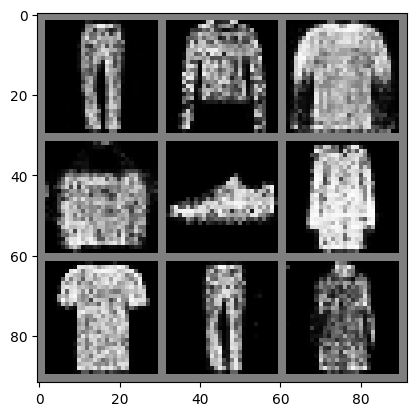
\includegraphics[width=.5\textwidth]{example_images.png}	
	\end{figure}

	\textcolor{red}{Here, you can make out the clothing items by their general shape, although the pixels are somewhat grainy.}

	\item Diversity of the generated images: Does the model generate a variety of clothing items?\\
	\textcolor{red}{ Yup, I made sure to set epsilon to a non-zero value, so the model should generate a variety of clothing items.
		In the above images, there are two t-shirts, two pairs of pants, and three long-sleeve shirts or dresses.
		There is also a purse (the square-shaped image).
	}

	\item Training stability: How stable are the loss curves? Are there signs of mode collapse?
 
	\textcolor{red}{The models' loss curves (D for discriminator, G for generator) are shown below:}
 
        \newpage

	\begin{figure}[t]
		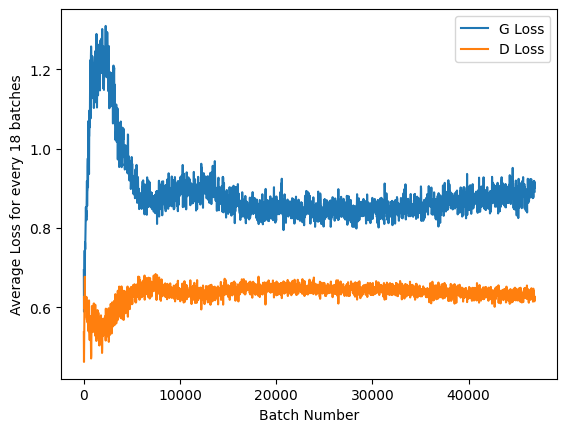
\includegraphics[width=.7\linewidth]{loss_chart.png}
	\end{figure}

	\textcolor{red}{The loss curves are pretty stable. The generator's loss is consistently higher than the discriminator's loss, which makes sense because the generator has to train more weights than the descriminator. 
		when the generator's loss spikes and the discriminator's loss drops, it indicates the generator is producing poor images.
		However, the loss curves quickly converge. There is partial mode collapse, since the generator is biased towards shirts and dresses (as seen in the generated images).
		Shirts and dresses are similar and more uniform in shape than other clothing items, so the generator is more likely to fool the discriminator with them.
		This leads to a partial mode collapse.
	}

\end{enumerate}

\end{document} 
